In this study, we analyze collision events recorded in a parallel universe where the Standard Model (SM) is nearly identical to ours. By examining events with a single jet plus missing transverse energy, as well as single jet plus muon pairs, we estimate the number of neutrino species in their SM.

The goal of this analysis is to estimate the number of neutrino species in the Standard Model of a parallel universe. Scientists there have built an analogue of the Large Hadron Collider (LHC) and performed proton-proton collisions at high energies. The primary focus is on the production and decay of the $Z$ boson, with particular interest in the decay channels $Z \to \nu \bar{\nu}$ and $Z \to \mu^+ \mu^-$. 


\section{Theory}
The $Z$ boson in this universe behaves similarly to ours, decaying into neutrinos and charged leptons. The key Feynman diagrams contributing to our signal processes are:

\begin{itemize}[label=\(\ \bigstar \)]
    \item $pp \to Z + \text{jet}$, followed by $Z \to \nu \bar{\nu}$.
    \item $pp \to Z + \text{jet}$, followed by $Z \to \mu^+ \mu^-$. 
\end{itemize}

\subsection{Feynman Diagrams}
In general we have the following Feynman diagram for \( pp \to f \bar{f} \) mediated by a \( Z \) boson:
\begin{figure}[H]
    \centering
    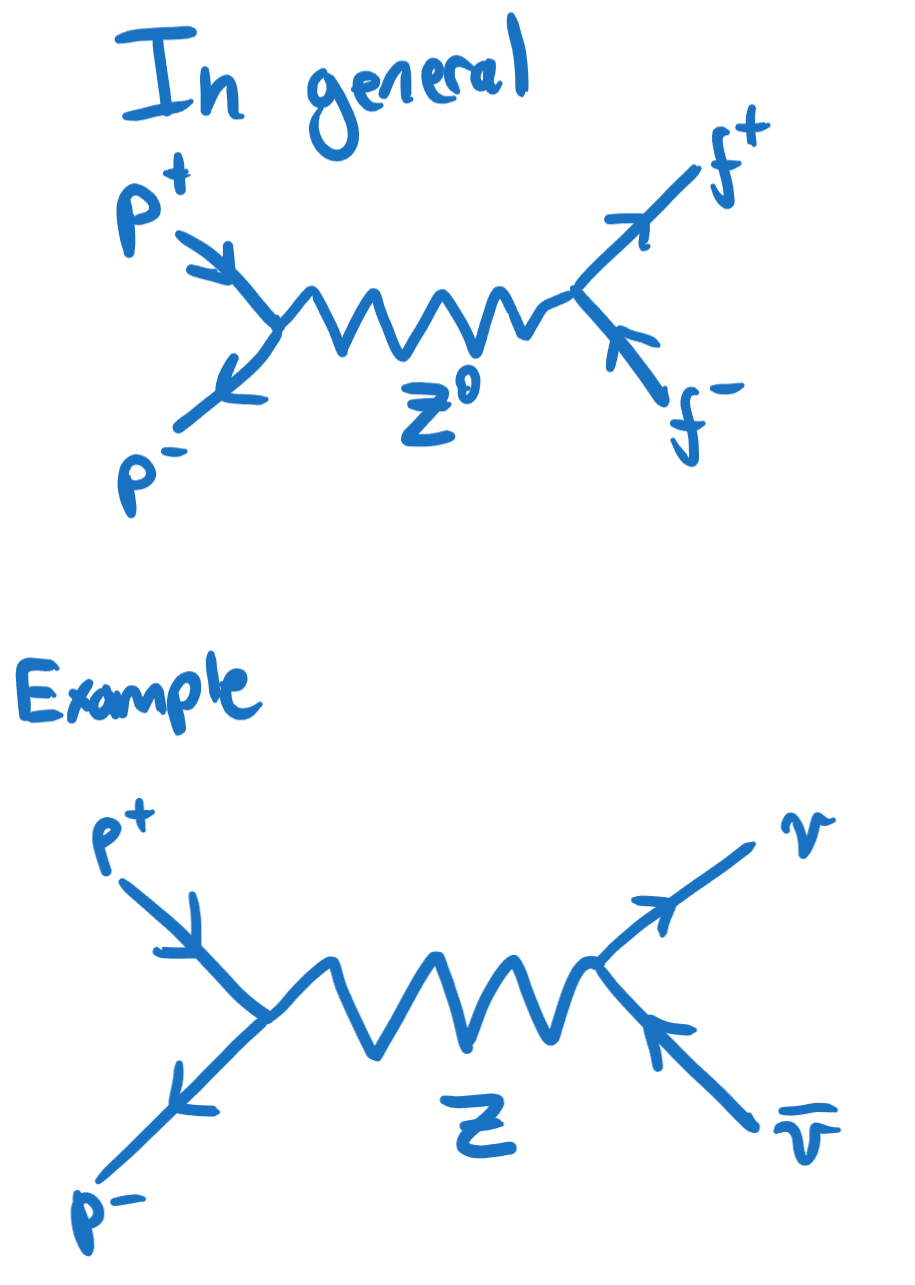
\includegraphics[width=0.45\textwidth]{AnalyzingColliderEvents/figures/ingeneral.png}
    \caption{Basic Feynman diagram for \( pp \to f \bar{f} \) mediated by a \( Z \) boson, and an example with neutrinos.}
\end{figure}

At the parton level, the dominant production mechanism is quark–antiquark annihilation: $q \bar{q} \to Z \to f \bar{f}$. Although gluons are abundantly produced in proton–proton collisions, they do not directly mediate the Z boson production, but can participate in initial or final state radiation that leads to additional jet activity. Once produced, the $Z$ boson decays into a fermion–antifermion pair. Depending on the decay channel, the fermion pair can consist of a neutrino pair or a muon pair. For our analysis, the muon pair serves as the signal, while the neutrino pair represents a background process. Although the $Z$ boson can decay into other fermion pairs, these are not relevant for our study.

In experimental analyses, the hadronic remnants associated with the quark or gluon that radiated the $Z$ boson are referred to as ``jets''. So the complete process is $pp \to Z + jets \to \mu \bar{\mu}$.

The presence of a jet in the event is often associated with the initial parton-level interaction.  For example, an initial state gluon can be emitted during the $q \bar{q} $ annihilation process, leading to the production of a $Z$ boson and a jet. This jet is a result of the fragmentation and hadronization of the outgoing parton.  The jet is a feature that accompanies both the signal (muon pair) and the background (neutrino pair) processes. We need to carefully consider the jet characteristics and any associated MET to distinguish between signal and background.

\begin{figure}[H]
    \centering
    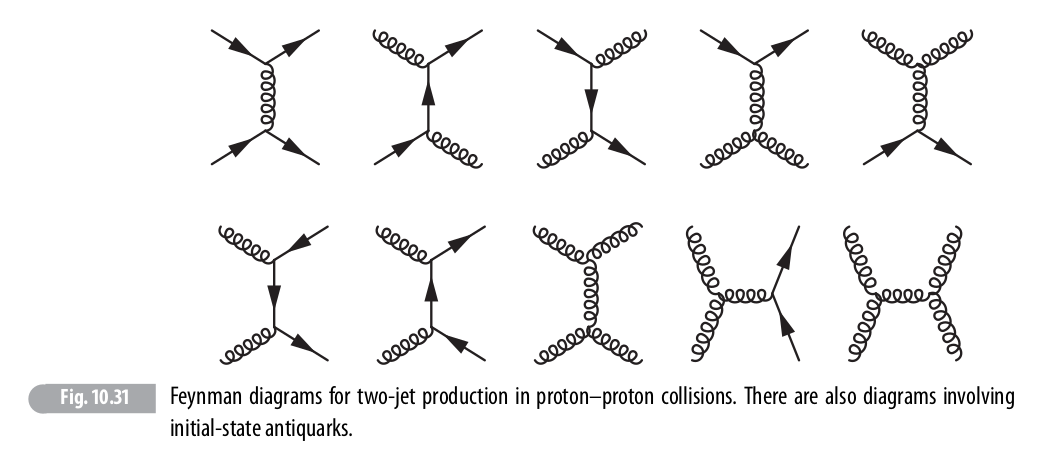
\includegraphics[width=0.45\textwidth]{AnalyzingColliderEvents/figures/Parton_pp.png}
    \caption{ From Thomson (2013), Modern Particle Physics. \cite{thomson} Showing the Feynman diagrams for two-jet production in a proton-proton collision.}
\end{figure}

Each diagram here illustrates a process where two outgoing partons (quarks or gluons) are produced. These partons will subsequently hadronize into two distinct jets. These diagrams are essentially the background processes for our $Z$ boson as they can mimic the jet production associated with the Z boson events. A finer example is: 

\begin{figure}[H]
    \centering
    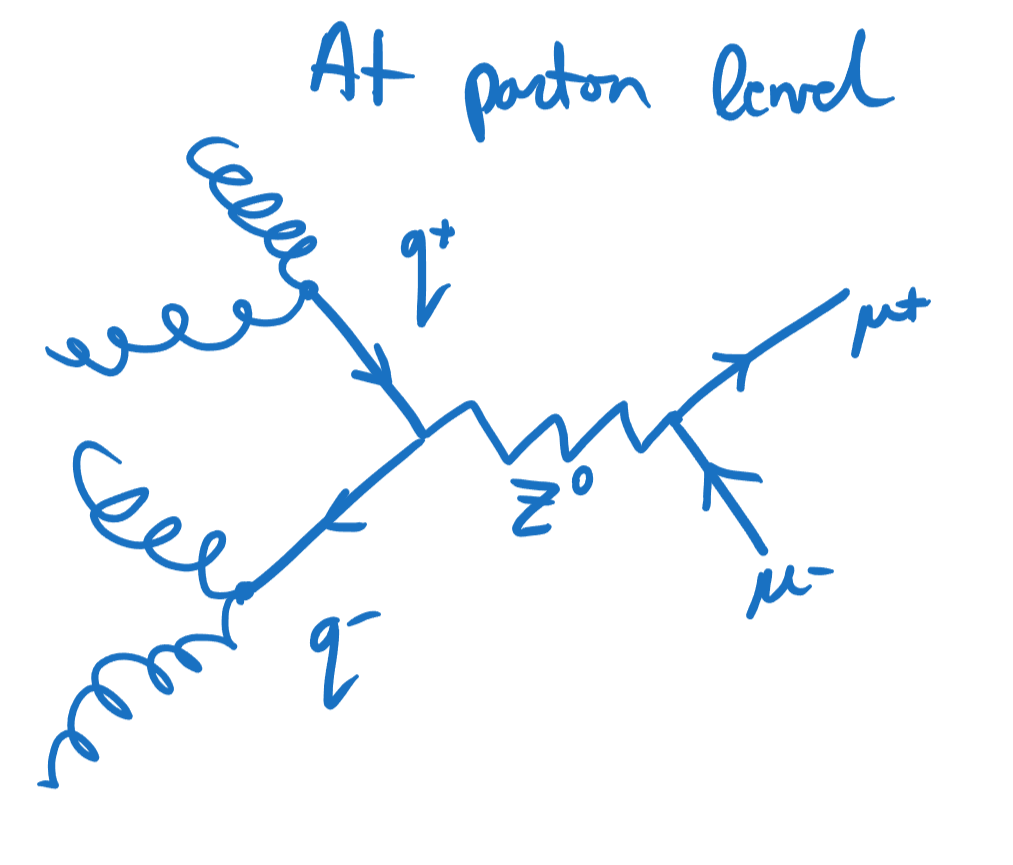
\includegraphics[width=0.45\textwidth]{AnalyzingColliderEvents/figures/examplebackground.png}
    \caption{An example background process that can occur}
\end{figure}

\subsubsection{Other processes not involving $Z$ Boson.}
The Drell-Yan process is a background process that contributes to the production of lepton pairs. It is a QED process and does not involve the $Z$ boson.

\begin{figure}[H]
    \centering
    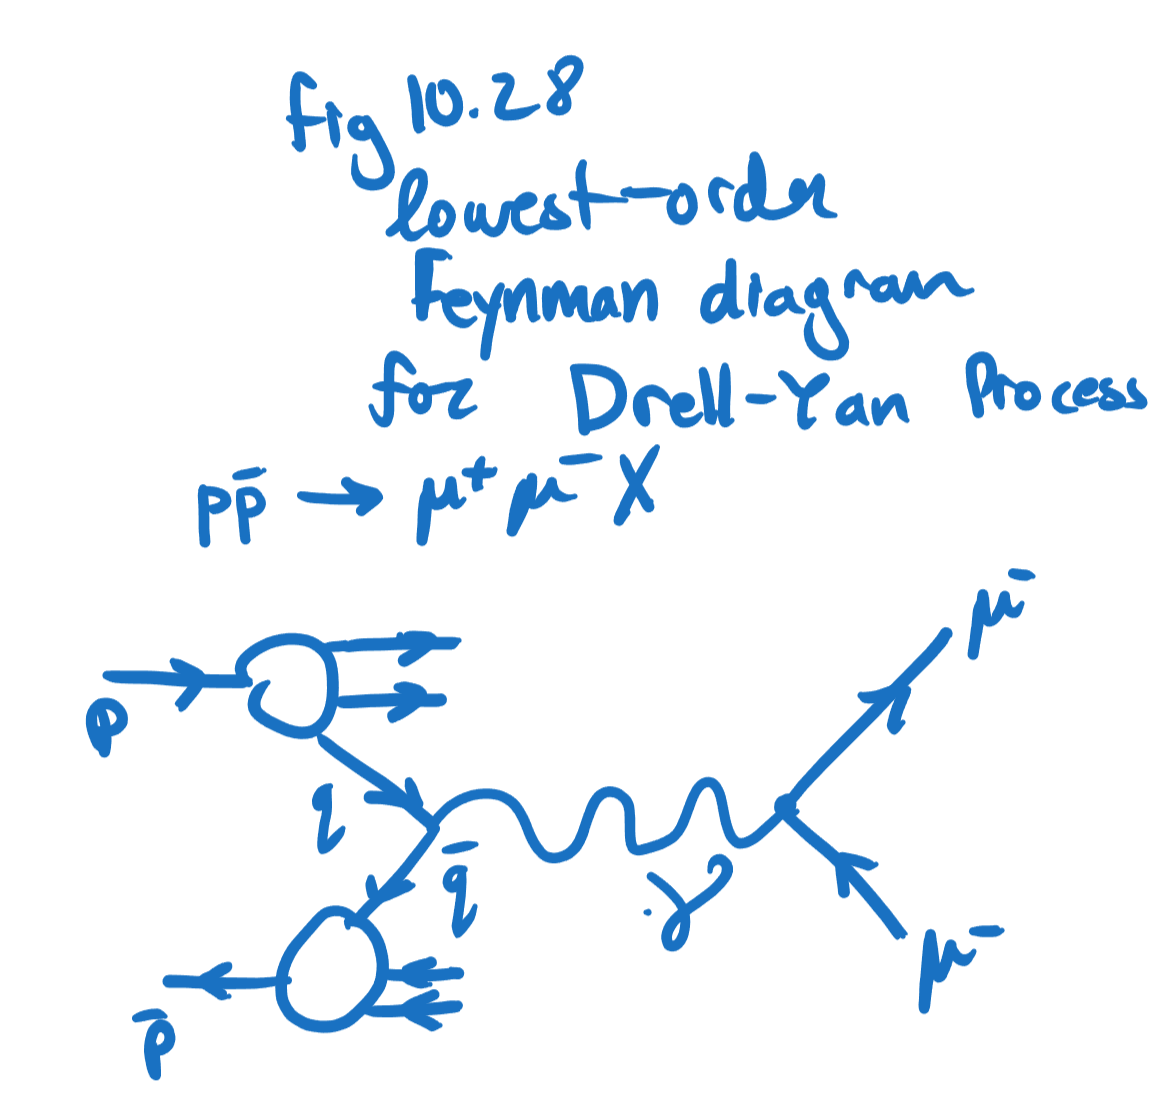
\includegraphics[width=0.45\textwidth]{AnalyzingColliderEvents/figures/drellyan.png}
    \caption{From \cite{thomson} Thomson (2013)  Modern Particle Physics. Showing the Feynman diagram for the Drell-Yan process.}
\end{figure}

\subsection{Isolate $Z$ Boson Contribution}

The amplitudes of the contributions to the final state \(mu^+ \mu^-\) should depend on the invariant mass of the $\mu^+ \mu^-$ pair by the following:
\begin{enumerate}
    \item $Z$ Boson contribution: The amplitude associated with our $Z$ boson process will have a Breit-Wigner distribution centered around the $Z$ boson mass ($m_Z \approx 91.2$ GeV).
    \begin{equation}
    A_{Z} \propto \frac{1}{(m^2_{\mu^+ \mu^-} - m^2_Z )^2 + (\Gamma_Z m_Z)^2} 
    \end{equation}
    \begin{itemize}[label=\(\ \star \)]
        \item $m_Z$ is the mass of the $Z$ boson.
        \item $\Gamma_Z$ is the width of the $Z$ boson.
    \end{itemize}
    \item Drell-Yan contribution: The amplitude associated with the Drell-Yan process will have a different dependence on the invariant mass
    \item The amplitude decreases with increasing mass further from the $Z$ boson mass.
    \begin{equation*}
        A_{Drell-Yan} \propto \frac{1}{m^2_{\mu^+ \mu^-}}
    \end{equation*}
\end{enumerate}

We can isolate the $Z$ boson contribution by selecting an invariant mass window, exploting the angular distributions, or using additional kinematic variables like rapidity or transverse momentum. An additional tool we can apply are machine learning algorithms to differentiate between events based on multivariate data inputs, identifying patterns specific to $Z$ decays versus other processes. 

For our project we will focus on the invariant mass window method and using the transverse momentum methods to enhance the purity of the $Z$ boson signal in our dataset.

\subsection{Why Require a Jet?}

Requiring a jet is experimentally \textbf{crucial}. In particular, for measuring the $Z \to \nu \bar{\nu}$ decay, the presence of a jet helps in reconstructing the event and distinguishing it from backgrounds. With the help of a jet---a collimated spray of particles resulting from a high-energy quark or gluon---we can detect the \textbf{invisible}. Neutrinos do not interact with the detector, so their presence is inferred by detecting an imbalance in the momentum in the plane transverse to the beam direction. This imbalance is called \textbf{Missing Transverse Energy (MET)}.

\subsection{Missing Transverse Energy (MET)}
We can measure the MET. Suppose a $Z$ is produced with little $p_T$ and decays into neutrinos. The resulting MET is small and very hard to distinguish from MET generated by detector mismeasurements or other background processes.

We can see this from the following equations:
\begin{equation}
    \text{MET} = -\sum_i \vec{p}_T^{\,i}
\end{equation}
where $\vec{p}_T^{\,i}$ represents the transverse momentum of visible particles in the event.

The jet's role in this process is that when a $Z$ is produced alongside a high-$p_T$ jet, the $Z$ itself must have a high $p_T$ to conserve momentum. When this high-$p_T$ $Z$ decays into neutrinos, the neutrinos carry away a significant amount of momentum, resulting in a large MET. This large MET, observed in conjunction with the high-$p_T$ jet, provides a much cleaner and more easily identifiable signal of $Z \to \nu \bar{\nu}$ decay.

We need to design a system can efficiently identify and measure this MET. This will allow the experiment to record the specific types of events out of the cast number of collisions. By selecting both $Z \to \nu \bar{nu}$ and $Z \to \mu^+ \mu^-$  events under similar kinematic conditions, we ensure we are comparing $Z$ bosons produced in a similar way. This will help us cancel uncertainties related to the  $Z$ production mechanism when calculating the ratio of the decay rates to estimate $N_{\nu}$.

\subsection{Strategy for Counting the number of Neutrinos}
We must examine the relationship between the $Z$ boson branching fractions to develop an analysis strategy. Our goal is to see how \text{BR}($Z \to \nu \bar{\nu}$) compares to \text{BR}($Z \to \mu^+ \mu^-$). In the standard model, the $Z$ boson couples to fermion-antifermion pairs ($f \bar{f}$). The strength of this coupling determines our partial decay width, $\Gamma(Z \to f \bar{f})$. If we assume the final state fermion masses are negligible compared to the $Z$ boson mass ($m_f << M_z$), we can see the partial width is given by:

\[
\Gamma (Z \to f \bar{f}) = N_c^f\frac{G_F M_Z^3}{6 \pi \sqrt{2}} \left[ \left(g_V^f\right)^2 + \left( g_A^f \right)^2 \right],
\]
\begin{itemize}[label=\(\ \star \)]
    \item $N_c^f$ is the number of colors for the fermion $f$ (1 for leptons, 3 for quarks)
    \item $G_F$ is the Fermi coupling constant
    \item $M_Z$ is the mass of the $Z$ boson
    \item $g_V^f$ and $g_A^f$ are the vector and axial-vector coupling constants for fermion $f$
\end{itemize}

The vector and axial-vector couplings of the fermion $f$ depend on the fermion's weak isospin $T_3^f$ and electric charge ($Q$) and are given by:
\begin{align}
g_V^f &= T_3^f - 2 Q \sin^2 \theta_W \\
g_A^f &= T_3^f,
\end{align} where $\theta_W$ is the weak mixing angle.

We can find these values from the PDG or calculate them. But the total width of the $Z$ boson is approximately 2.495 GeV, the partial width for each charged lepton is 83.99 MeV. The partial width for each neutrino species is 167.21 MeV.

So the branching ratio of $Z \to \nu \bar{\nu}$ is:

\[
BR(Z \to \nu \bar{\nu}) = N_\nu \times \frac{ 167.21 \text{ MeV}}{2.495 \text{ GeV}}\]

where $N_\nu$ is the number of neutrino species.

The branching ratio of $Z \to \mu^+ \mu^-$ is:

\[
BR(Z \to \mu^+ \mu^-) = \frac{ 83.99 \text{ MeV}}{2.495 \text{ GeV}}
\]
The ratio between the Neutrino and Muon decay is:

\[
\frac{BR(Z \to \nu \bar{\nu})}{BR(Z \to \mu^+ \mu^-)} = N_\nu \times \frac{167.21}{83.99} \approx 2N_\nu
\]
This means that the ratio of the observed (jet +missing energy) to the expected (jet + $\mu^+ \mu^-$) events should be approximately twice the number of neutrino species.

\section{Analysis Method}
To estimate the number of light neutrino species \( N_\nu \), we analyze the ratio of two event types: those with visible muon pairs and those with significant missing transverse energy (\( E_T^{\text{miss}} \)), attributed to neutrinos.

The relevant processes are:
\begin{align*}
pp &\to Z + \text{jet} \to \mu^+ \mu^- + \text{jet}, \\
pp &\to Z + \text{jet} \to \nu \bar{\nu} + \text{jet}.
\end{align*}


Since the Z boson decays democratically into all neutrino flavours, the total invisible decay rate is proportional to the number of neutrino generations:
\begin{equation}
\Gamma(Z \to \text{invisible}) = N_\nu \cdot \Gamma(Z \to \nu_\ell \bar{\nu}_\ell).
\end{equation}

We define the ratio of observed event counts as:
\begin{equation}
R = \frac{N_{\text{jet} + E_T^{\text{miss}}}}{N_{\text{jet} + \mu^+ \mu^-}} \approx \frac{\text{BR}(Z \to \nu \bar{\nu})}{\text{BR}(Z \to \mu^+ \mu^-)}.
\end{equation}

Given that each neutrino flavour contributes equally and the partial width \( \Gamma(Z \to \mu^+ \mu^-) \) is known, we obtain:
\begin{equation}
N_\nu = R \cdot \frac{\Gamma(Z \to \mu^+ \mu^-)}{\Gamma(Z \to \nu_\ell \bar{\nu}_\ell)}.
\end{equation}

Using Standard Model values:
\[
\frac{\Gamma(Z \to \mu^+ \mu^-)}{\Gamma(Z \to \nu_\ell \bar{\nu}_\ell)} \approx \frac{1}{0.5} = 2,
\]


we get the practical estimate:
\begin{equation}
N_\nu \approx \frac{R}{2}.
\end{equation}

This method allows us to extract the number of neutrino generations present in the model underlying the dataset, assuming all other decay channels are either known or negligible in this sample.

With our selection strategy validated, we proceed to apply the cuts to both datasets and analyze the estimated number of neutrino species.

\subsection{Kinematic Cuts}
We are going to apply selection rules to the events based on some kinematic properties of the particles in the detector. Our goal is to isolate the clean signals from noisy backgrounds so we can ensure reliable detector performance. This will allow us to focus our analysis on regions where the model is valid. Some quantities that can we use for the cuts are:
\begin{table}[ht]
    \centering
    \begin{tabular}{|c|c|}
    \hline
    \textbf{Quantity} & \textbf{Description} \\
    \hline
    $p_T$ & Transverse Momentum \\
    $E^{miss}_T$ & Missing Transverse Energy \\
    $\eta$ & Pseudorapidity (angle with respect to beam axis) \\
    $\phi$ & Azimuthal Angle \\
    $m_{\mu \mu}$ & Invariant Mass of the Muon Pair (can be used to identify $Z$ boson) \\
    \hline
    \end{tabular}
    \label{tab:key_quantities}
    \end{table}

Our events are going to be:
\begin{align*}
    pp &\to Z + \text{jet} \to \mu^+ \mu^- + \text{jet}, \\
    pp &\to Z + \text{jet} \to \nu \bar{\nu} + \text{jet}.
    \end{align*}
Some of our $\mu^+ \mu^-$  events may have low transverse momentum or lie outside the detector acceptance region. Our jets may also be from other QCD processes or just noise. So by applying kinematic cuts, we can ensure that only high-quality muons and jets are considered. Our events have well measured MET and biases from detector limits get reduced.

Examples of kinematic cut are:
\begin{enumerate}
    \item Jet transverse momentum cut, keep only jets with $p_T > 30$ GeV. This ensures that the jets are energetic enough to be detected and are likely to be from the hard scattering process and not from QCD background.
    \item Muon transverse momentum cut, keep only muons with $p_T > 20$ GeV. This ensures that the muons are energetic enough to be detected and are likely to be from the $Z$ boson decay.
    \item MET significance cut, require $E^{\text{miss}}_T > 30$ GeV. This ensures that the missing transverse energy is significant enough to be detected and is likely to be from the neutrinos.
    \item Invariant mass window, require $ 81 \text{ GeV} \leq m_{\mu^+ \mu^-} \leq 101$ GeV. This ensures that the muons are from the $Z$ boson decay and are related to the neutrino branching. 
\end{enumerate}
\subsubsection{Verifying our Methods}
We can start by verifying our data by plotting the invariant mass of the muon pairs. We expect to see a peak around the Z boson mass of 91.1876 GeV. This is a good way to verify that our data is correct. 

\begin{figure}[H]
    \centering
    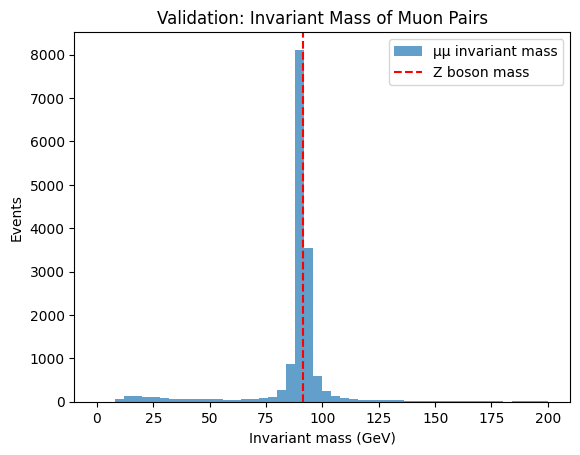
\includegraphics[width=0.8\textwidth]{AnalyzingColliderEvents/figures/muonmass.png}
    \caption{Muon Pair Invariant Mass Distribution}
    \label{fig:muon_pair}
\end{figure}

So we can see that we have a peak around 91.1876 GeV, which is the mass of the Z boson. This is a good sign that our data is correct.

To do a cross check validation of our methods, we are going to be plotting the MET before and after the cut to see signal improvement. We will also check the transverse momentum balance in visible events. If the transverse momentum is balanced we should expect values to cancel out. 
So in these next figures we have the MET before and after:

\begin{figure}[H]
    \centering
    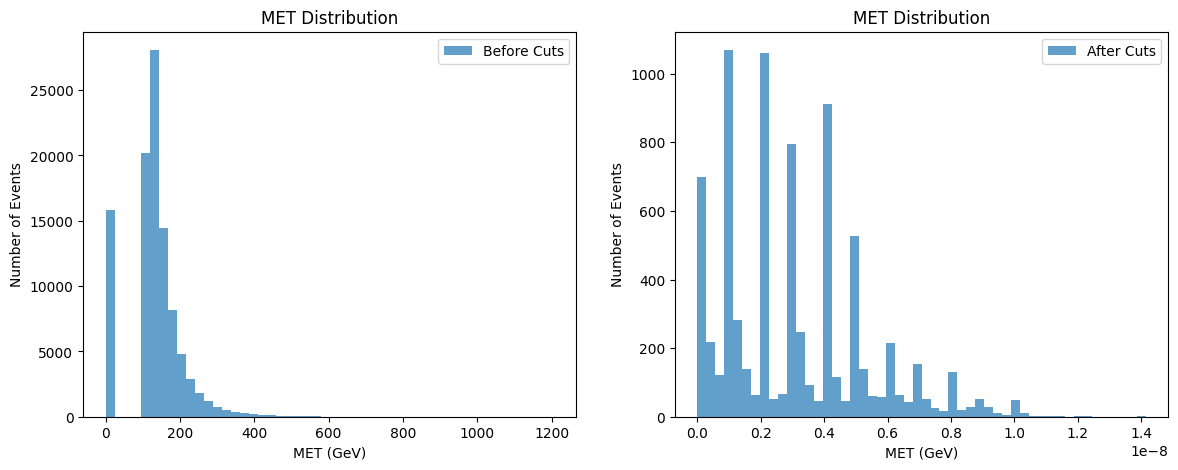
\includegraphics[width=0.8\textwidth]{AnalyzingColliderEvents/figures/MET.png}
    \caption{MET Distribution before and after the cut}
    \label{fig:MET_before}
\end{figure}
Here we can see that MET after the cut is significantly lower than before the cut. This is a good sign that our cuts are working as expected.

For our methods we will also be employing different combinations of kinematic cuts. The first method will apply all the kinematic cuts. We will try different combinations (by simply commenting out the cuts we want and don't want) to see how the results change. Since we are given dataset with our universe (where we expect $N_{\nu} = 3$) we can use this to verify our methods. Once we decide on the cuts that get us to the closest result we will apply them to the other dataset from the other universe. 

After testing the different combinations, we find that the best results are obtained with the following cuts:
\begin{lstlisting}
another_universe_selected_events = []

for event in another_universe_sample_data:
    if 'muons' not in event:
        continue

    muons = event['muons']
    if len(muons) != 2:
        continue  # Require two muons

    # Kinematic cuts
   # if not all(pT(mu) > 20 for mu in muons):
     #   continue  # Both muons must have pT > 20 GeV
   # if not all(abs(eta(mu)) < 2.5 for mu in muons):
     #   continue  # Within detector acceptance

    # Invariant mass cut around Z peak
    mass = invariant_mass(muons[0], muons[1])
    if not (80 < mass < 100):
        continue

    another_universe_selected_events.append(event)
\end{lstlisting}
which means that we are only selecting events have muons and the invariant mass of the muons is between 80 and 100 GeV.
\section{Results}
\subsection{Prior to any kinematic cuts}
Prior to doing any Kinematic cuts, we find that: 
\begin{lstlisting}
# Count events with muons and without
n_visible = 0
n_invisible = 0

for event in sample_data:
    if 'muons' in event:
        n_visible += 1
    else:
        n_invisible += 1

# Estimate the number of neutrino flavours
ratio = n_invisible / n_visible
N_nu = ratio / 2
print(f"Visible (muons) events: {n_visible}")
print(f"Invisible (neutrino) events: {n_invisible}")
print(f"ratio: {ratio:.2f}")

print(f"Estimated number of neutrino species: {N_nu.3f}")
        \end{lstlisting}

\subsection{Analysis}

We find that $N_\nu \approx 2.66$ prior to doing any kinematic cuts for our universe.  For the other universe dataset, we get the results: $N_\nu \approx 3.55$



\subsection{Kinematic Cuts}

The following code is only an example of the kinematic cuts we used to filter the data.  We used a variety of cuts to filter the data.
\begin{lstlisting}
selected_events = []

for event in sample_data:
if 'muons' not in event:
    continue

muons = event['muons']
if len(muons) != 2:
    continue  # Require two muons

# Kinematic cuts
if not all(pT(mu) > 20 for mu in muons):
    continue  # Both muons must have pT > 20 GeV
if not all(abs(eta(mu)) < 2.5 for mu in muons):
    continue  # Within detector acceptance

# Invariant mass cut around Z peak
mass = invariant_mass(muons[0], muons[1])
if not (80 < mass < 100):
    continue

selected_events.append(event)

n_visible = len(selected_events)
n_invisible = sum(1 for event in sample_data if 'muons' not in event)

R = n_invisible / n_visible
N_nu = R / 2

print(f"Selected visible (Z to mu mu) events: {n_visible}")
print(f"Invisible (Z to nu nu) events: {n_invisible}")
print(f"Ratio R = {R:.2f}")
print(f"Estimated number of neutrino flavours: N_nu = {N_nu:.2f}")

\end{lstlisting}

\subsection{Post-cut Analysis}

After applying the cuts we find our universe has $N_\nu \approx 3.15$ and the other universe has $N_\nu \approx 4.26$

After applying the kinematic cuts, the number of selected events that pass these criteria changes, affecting our estimate for the number of neutrino flavors in the other universe.


\begin{enumerate}
    \item The ratio \(R\) increased significantly post-cuts. This implies that the number of selected visible events has decreased more substantially than the invisible ones, likely because the cuts effectively filter out only the cleanest signals of \(Z \to \mu^+\mu^-\) decays.
    \item The post-cut estimate for $N_\nu$ in the other universe is \(N_\nu = 4.26\). This value significantly deviates from the value of 3 in our universe. This discrepancy could suggest  fundamental particle interactions in the other universe being different.
    \item The kinematic cuts, by design, should reduce background and focus purely on \(Z \to \mu^+\mu^-\) decays; however, the decrease in visible events also reflects stringent selectivity, ensuring only events well within the accepted physical and detector bounds contribute.
\end{enumerate}

We find that $N_\nu \approx 4.26$ after applying kinematic cuts. Assuming this discrepancy from the canonical three neutrino species isn't due to methodological errors, this result hints at intriguing differences in the underlying particle physics of the parallel universe compared to our own. Here are some possible implications:

\begin{itemize}[label=\(\ \star \)]
    \item  The increased estimate could suggest the existence of additional neutrino-like particles, perhaps with weaker coupling to the \(Z\) boson, thus contributing differently to its decay width.
    \item  Higher effective neutrino counts may reflect enhanced coupling constants or exotic phenomena  that don't interact directly like standard model neutrinos but have indirect effects.
    \item  The electroweak symmetry breaking mechanism could differ, influencing \(Z\) boson decay dynamics and increasing the apparent number of neutrino species beyond our familiar three-generation model.
  
    \item  Should these findings hold, cosmological models in this universe would likely differ, affecting nucleosynthesis and cosmic microwave background patterns due to variations in particle contributions to the universe's mass-energy content. Once again, from the Big Bang to the present day, the universe's evolution would be influenced by these differences.
\end{itemize}

These post-cut results encourage further exploration of potential physics beyond the Standard Model we observe, offering new avenues for theoretical and experimental inquiry into the nature of this parallel reality.

An increased \(N_\nu\) could mean that either the parallel universe features more neutrino-like particles or a fundamentally different electroweak interaction symmetry structure. Understanding why these effectively higher neutrino counts occur might require revisiting assumptions about relative neutrino-decay widths or investigating new physics scenarios allowing for additional neutrino-like degrees of freedom.

Some further investigations that we could employ to better understand these results include:
\begin{itemize}[label=\(\ \star \)]
\item Re-evaluating cut parameters and simulations might help deduce if hardware (detector range and efficiency simulations) plays a role in these shifts.
\item Cross-checks with additional decay channels and collider event types might provide further insight into confirmation or deviation from expected physics in this parallel universe.
\end{itemize}
By carefully reviewing and interpreting these results, we can frame a more comprehensive understanding of discrepancies introduced due to either the physical properties of the particles involved or the constraints imposed by your experimental or data assumptions.

An interesting after-thought would be what if we had less than 3 neutrino species in an universe? This would imply that the universe is fundamentally different from what we observe. For example, if we assume that this is an inherent property of the parallel universe and not due to some error or methodological issue. This could imply some interesting differences in the fundamental properties of their physics compared to our universe. For example:
\begin{itemize}[label=\(\ \star \)]
    \item The existence of fewer neutrino flavours can imply that the existing particles do not contribute equally to the $Z$ boson decay width. This could stem from the differences in couplings or symmetries in the universe's version of the Standard model
    \item This universe might also feature additional neutrino-like particles that do not interact like our typical standard model neutrinos. These particles would contribute partially to the decay width which results in the effective count of neutrino species being less than 3.
    \item The dynamics of the electroweak symmetry breaking might be different which causes the $Z$ boson to decay differently. 
    \item Cosmology itself might be different in this universe due to differences in energy density in the early universe. Post the Big Bang, the universe might have formed completely differently than ours.
\end{itemize}